	\subsection{Problem 1a}
	
	\bigskip
 Dynamical systems are mathematical objects used to model physical phenomena whose state (or instantaneous description) changes over time. These models are used in financial and economic forecasting, environmental modeling, medical diagnosis, industrial equipment diagnosis, and a host of other applications.
    To study dynamical systems mathematically, we represent them in terms of differential equations.
    
    The state of dynamical system at an instant of time is described by a point in an n-dimensional space called the \textbf{state space} (the dimension n depends on how complicated the systems is) . As time passes the point moves, sweeping out a curve in the state space, called a \textbf{trajectory} of the system (mathematically, this curve is a solution of the governing differential equations)
   
    A system can be classified according to different criteria, such as
    
    \bigskip
\begin{table}[h]
\centering
\begin{tabular}{|c|c|}
\hline
\multicolumn{2}{|c|}{System Classification}     \\ \hline
\textit{\textbf{Either}} & \textit{\textbf{Or}} \\ \hline
Deterministic            & Stochastic           \\ \hline
Discrete                 & Continous            \\ \hline
Linear                   & Nonlinear            \\ \hline
Autonomous               & Nonautomonous        \\ \hline
\end{tabular}%

\end{table}
\bigskip
\bigskip
    
A deterministic system has an entirely predictable behavior. The system is fully understood, and it is possible to predict exactly what will happen. A stochastic model, on the other hand, possess inherent randomness that make it impossible to predict its behavior. 

A discrete system changes the state variables only at a countable number of points in time. Dynamical systems with discrete time, like the ideal coin toss, have their states evaluated only after certain discrete intervals. In the case of the coin toss, the smooth tumbling and bouncing of the coin is ignored, and its state is only viewed when it has come to equilibrium. These points in time are the ones at which the event occurs/change in state. A continuous system, however, change in a continuous way, and not abruptly from one state to another, ex: A pendulum swinging back and forth,...

In a linear system, function describing the system behavior must satisfied 2 basic properties:

\[Addictivity: f(x+y)=f(x)+f(y)\]
\[Homogeneity: f(\alpha x) = \alpha f(x)\]

A nonliner system's function simply doesn't satisfied the above requirements.

An autonomous system is a system of ordinary differential equations, which do not depend on the independent variable. If the independent variable is time, we call it time-invariant system.

A nonautonomous system is a system that doesn't satisfied the above requirements.

In this assignment, we use the dynamical system especially the first order differential equation to predict the changes of CO2 inside a greenhouse model


\subsection{Problem 1b}
The first order differential equations in the dynamical system with the initial value $y_0$ and $t_0$ can be re-written as:
\[
\left\{\begin{array}{ll}
\frac{dy}{dx} & =f(x, y) \\
y\left(x_{0}\right) & =y_{0}
\end{array}\right.
\]

Suppose we have a linear differential equation 
\[y+p(x)y=g(x)\] in which p and g are continous functions on the open interval I = $(\alpha,\beta)$. Then for each $t \in I$ there exists a unique solution $y=\phi(t)$ to the differential
equation $\frac{dy}{dx}+p(x)y=g(x)$  that also satisfies the initial value condition $y(x_0)=y_0$
\subsection{Problem 1c}

A differential equation is an equation which contains one or more terms and the derivatives of one variable (i.e., dependent variable) with respect to the other variable (i.e., independent variable). The order of the equation is equal to the highest order of the derivative in the equation, therefore a first-order differential equation only have first-order derivative in their equation

\[\frac{dy}{dx} = f(x)\]

We often have to find a particular solution which specifies the value of the unknown function at a given point in the domain. This is called an initial-value problem.
For example, solve the diferential equation:

\[\Dot{y} = 2(25-y)\] Knowing that
\[y(0) = 40\]

We can see that if y(t) = 25 then it will satisfy the first equation but y(0) = 25 $\neq$ 40. So y(t) = 8 is not a solution. So as long as y is not 8, we can rewrite the equation as

\[\frac{dy}{dt}\frac{1}{25-y} = 2 \]
\[\Leftrightarrow \frac{1}{25-y}dy =2dt\]
\[\Leftrightarrow  \int \frac{1}{25-y} dy = \int 2dt\]
\[\Leftrightarrow ln\lvert 25 - y\rvert * (-1) = 2t + C_0\]
\[\Leftrightarrow ln\lvert 25 - y\rvert = -2t - C_0 = -2t + C\]
\[\Leftrightarrow \lvert 25 - y\rvert = e^{-2t+C}\]
\[\Leftrightarrow y - 25 = \pm  e^C e^{-2t}\]
\[\Leftrightarrow y = 25 \pm e^C e^{-2t} = 25 + Ae^{-2t}\]

A is some non-zero constant. Since we want y(0) = 40, we substitute and solve for A:
\[40 = 25 + Ae^0\]
\[A = 15\]
Thus $y = 25 + 15e^{-2t}$ is the solution of the differential equation.

\subsection{Problem 1d}
\begin{itemize}
    \item Explicit Euler
\end{itemize}
In mathematics and computational science, the Euler method (also called forward Euler method) is a first-order numerical procedure for solving ordinary differential equations (ODEs) with a given initial value. It is the most basic explicit method for numerical integration of ordinary differential equations and is the simplest Runge–Kutta method. 

Explicit methods calculate the state of the system at a later time from the state of the system at the current time without the need to solve algebraic equations. For the method, we begin by choosing a step size or $\Delta t$. The size of $\Delta t$ determines the accuracy of the approximate solutions as well as the number of computations. Graphically this method produces a series of line segments, which thereby approximates the solution curve. 

Given $\frac{dy}{dt}=f(t,y)$ with $y(t_0)=y_0$ we approximate the path of the solution by:

\begin{enumerate}
    \item Step size:  First, we choose the step size $h$ which is the size of the increments along the t-axis that we will use in approximation. Smaller increments tend to give more accurate answers, but then there are more steps to compute. 
    \item Compute slope: Compute the slope $\frac{dy}{dt} = f(t_0,y_0)$
    \item Get next point: The next point is $t_1 = t_0 + h$ and $y_1 = y_0 + f(t_0,y_0)h$
    \item Repeat: : Repeat the last two steps with $(t_1,y_1)$
\end{enumerate}
\begin{figure}[h]
    \centering
    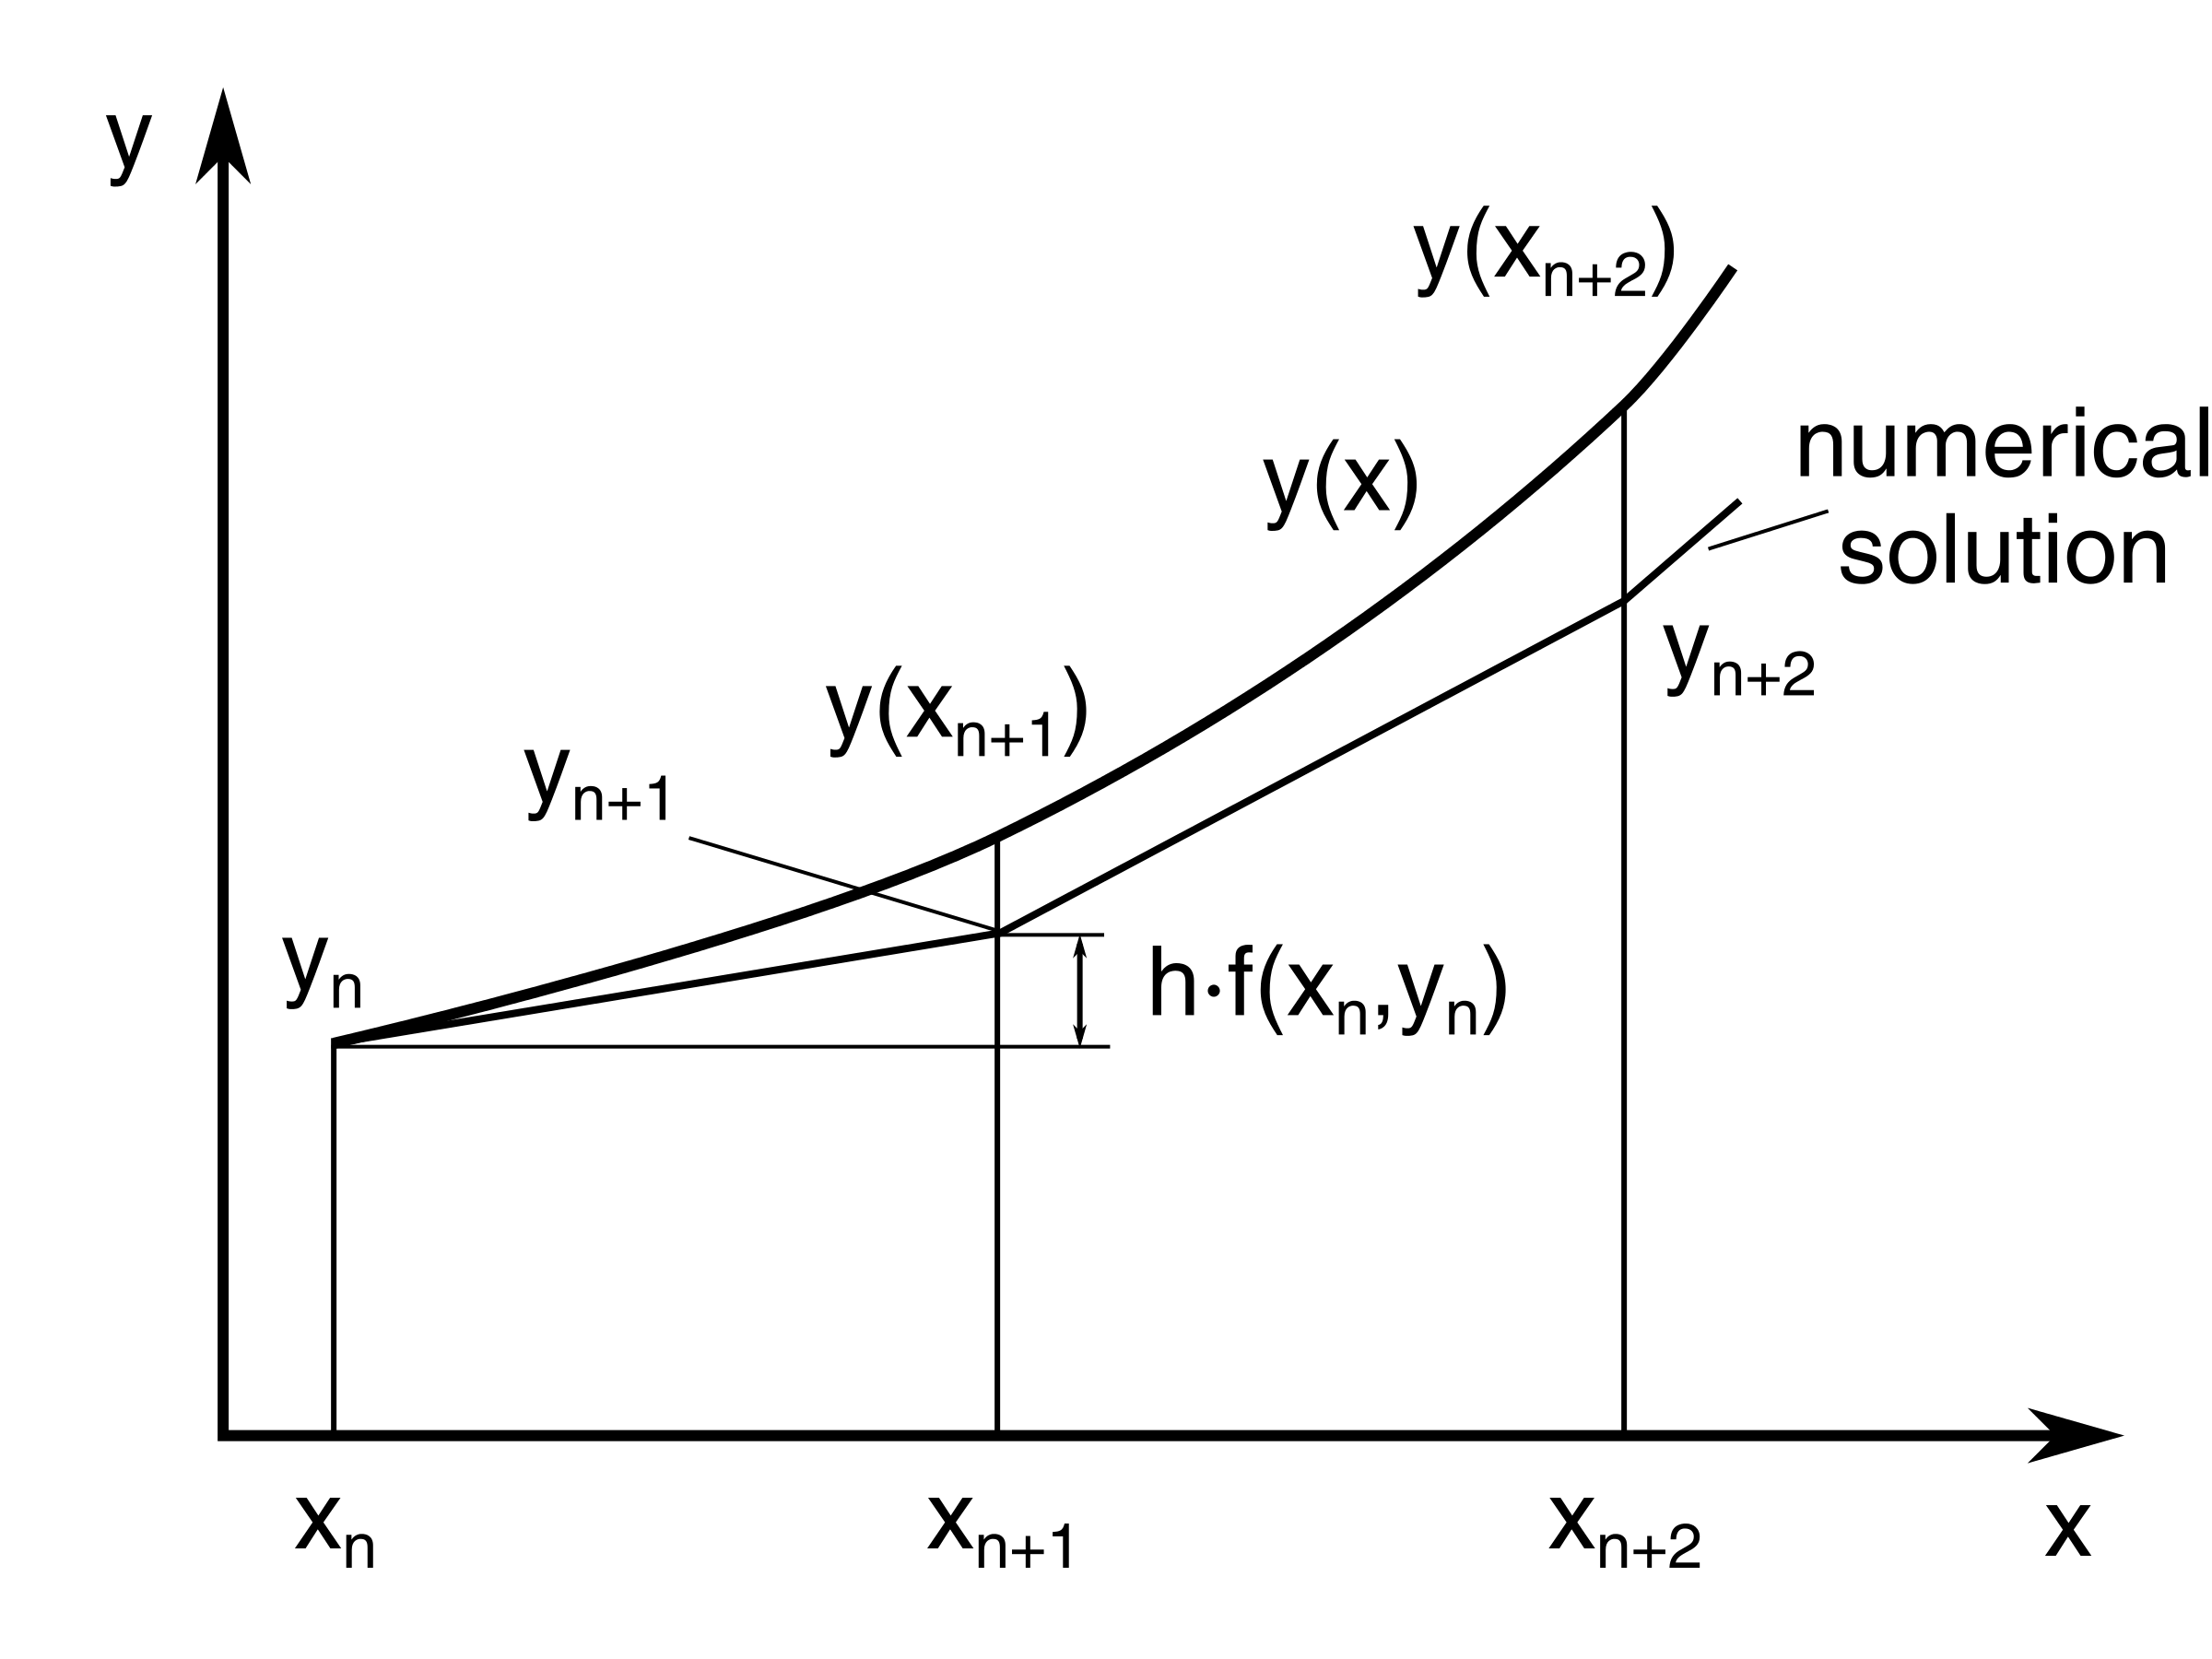
\includegraphics[width = 2in, height = 2in]{Code/Pic/Euler.png}
    \caption{Explicit Euler metho}
    \label{fig:my_label}
\end{figure}
\begin{itemize}
    \item Explicit Runge–Kutta of order 4
\end{itemize}
In numerical analysis, the Runge–Kutta methods are a family of implicit and explicit iterative methods, which include the well-known routine called the Euler Method, used in temporal discretization for the approximate solutions of ordinary differential equations. The most widely known member of the Runge–Kutta family is generally referred to as "RK4", the "classic Runge–Kutta method" or simply as "the Runge–Kutta method".

Supoose we have a problem: $\frac{dy}{dt}=f(t,y)$ with $y(t_0)=y_0$
With y is an unknown function (scalar or vector) of time $t$,  which we would like to approximate. We also know the rate of change $\frac{dy}{dt}$ is a function of y and t; and the initial value.
 First,  we choose the step sizehwhich is the size of the increments along thet-axis that we will use in approximation. We define
 \[y_{n+1}=y_n+\frac{1}{6}h(k_1+2k_2+3k_3+4k_4\]
 \[t_{n+1}=t_n+h\]
 for n = 0,1,2,3,..... with
 \[k_1=f(t_n,y_n)\]
 \[k_2=f(t_n+\frac{h}{2},y_n+h\frac{k_1}{2})\]
 \[k_3=f(t_n+\frac{h}{2},y_n+h\frac{k_2}{2})\]
 \[k_4=f(t_n+h,y_n+h k_3)\]
 Here, by using the RK4 approximation, we get the next value $y_{n+1}$ using present value $y_n$ and the weighted average of four increments, where each increment is the product of the size of the interval, h  and an estimated slope specified by function f on the right-hand side of the differential equation.
 
$k_1$  is the slope at the beginning of the interval, using y (Euler's method).

$k_2$ is the slope at the midpoint of the interval, using $y$ and $ k_1$.

$k_3$ is also the slope at the midpoint, but now using $y$ and $k_2$.

$k_4$ is the slope at the end of the interval, using $y$ and $k_3$

\noindent    In averaging the four slopes, greater weight is given to the slopes at the midpoint. 
\subsection{Problem 1e}  

Given that,
\[\Dot{y} = 2(25-y)\] and
\[y(0) = 40\]

Find y(0.1)

We know the solution is $y = 25 + 15e^{-2t}$. We choose h = 0.1

\textbf{Euler method}: 
\begin{align*}
   y(0.1) &= y_0+hf(y_0,t_0)\\
        &= 40+0.1(2(25-40))\\
        &= 37
\end{align*}

\textbf{RK4 method}:
\[k_1=2(25-40)=-30\]
\[k_2=2(25-38.5)=-27\]
\[k_3=2(25-38.65)=-27.3\]
\[k_4=2(25-37.2)=-24.54\]


$y(0.1) = y(0)+\frac{1}{6}h(k_1+2k_2+3k_3+4k_4)=36.599$



True y(0.1) = $25+15e^{-2*0.1} \approx 37.28 $

